\begin{figure}
    \centering
    \begin{subfigure}{0.48\textwidth}
        \centering
        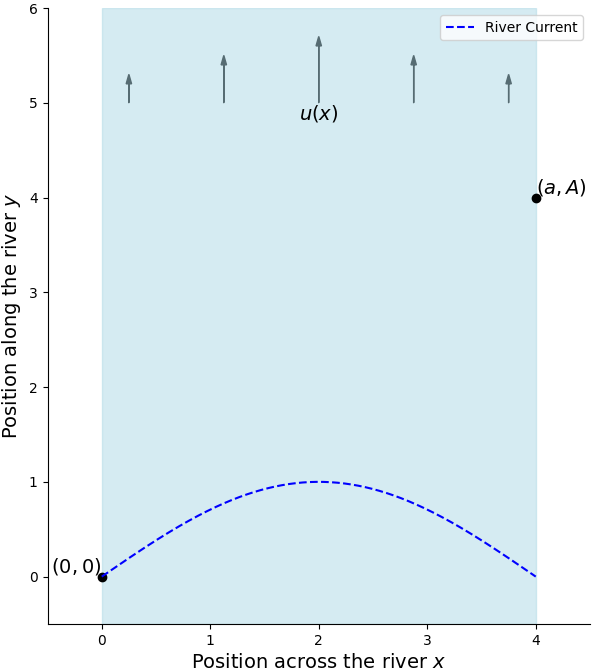
\includegraphics[width=\textwidth]{papers/schwimmen/Grafiken/Figure_2-crop.png}	
        \caption{Flussströmung}
        \label{fig:no_velocity}
    \end{subfigure}
    \hfill  
    \begin{subfigure}{0.48\textwidth}
        \centering
        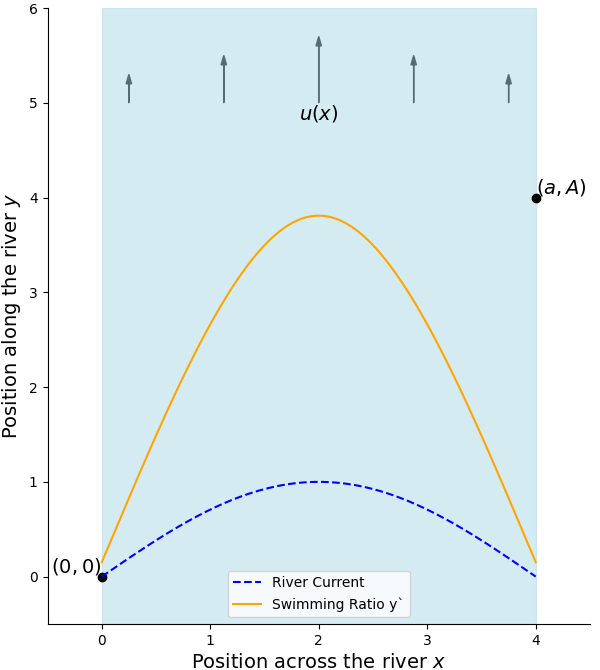
\includegraphics[width=\textwidth]{papers/schwimmen/Grafiken/Figure_3-crop.png}	
        \caption{\(y' = \frac{dy}{dx}\)}
        \label{fig:diagonal_velocity}
    \end{subfigure}
    \par\bigskip
    \begin{subfigure}{0.48\textwidth}
        \centering
        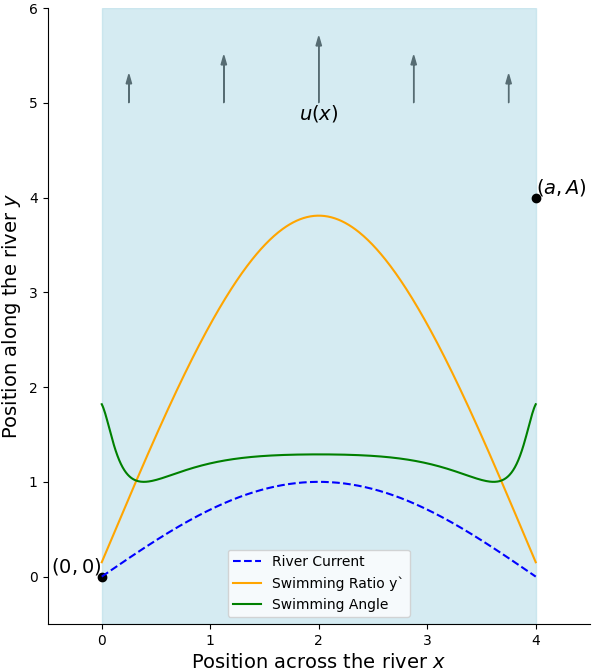
\includegraphics[width=\textwidth]{papers/schwimmen/Grafiken/Figure_4-crop.png}	
        \caption{Winkel der Schwimmenden Person}
        \label{fig:squerd_velocity}
    \end{subfigure}
    \hfill  
    \begin{subfigure}{0.48\textwidth}
        \centering
        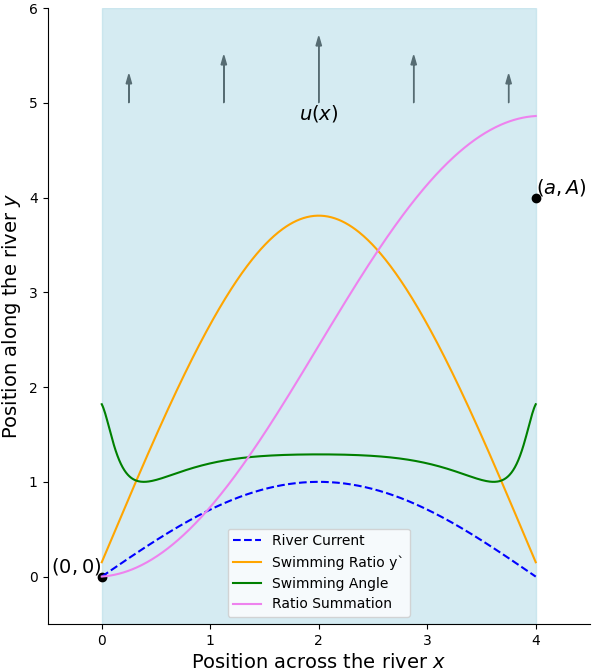
\includegraphics[width=\textwidth]{papers/schwimmen/Grafiken/Figure_5-crop.png}	
        \caption{Aufsumierte Steigung}
        \label{fig:sin_velocity}
    \end{subfigure}
    \par\bigskip
    \caption{Die vier Grafiken stellen verschiedene Graphen dar die für die Flussüerquerung zentrall sind, \((a)\) stellt die Flussströmung dar, \((b)\) das Verhältis zwischen was in \(x\)- und \(y\)-Richtung geschwommen wird, \((c)\) den Winkel der aus dem Verhältnis folgt und \((d)\) das aufsummierte Verhältnis}
    \label{fig:river_pfrofiles}
\end{figure}
